\documentclass{article}

% Add necessary packages
\usepackage{natbib, graphicx, fancyhdr} % For managing references
\usepackage{titlesec} % For customizing section titles
% natbib for bibtext

% Add necessary commands
\bibliographystyle{plainnat} % Specify the bibliography style

% Define margins
\usepackage[margin=2.5cm]{geometry}

\graphicspath{{images/}} % Configuring the graphicx package

% Define header and footer
\pagestyle{fancy}
\fancyhf{}
\lhead{
\includegraphics[height=.65cm]{etsiit-1.png}}
\rhead{\textbf{\textit{PinguAR}}}
\cfoot{\textbf{\textit{\thepage}}}
\renewcommand{\headrulewidth}{0.7pt}
\setlength{\headheight}{23pt}

% This is to define a style with no footer for the table of contents
\fancypagestyle{nofooter}{%
  \fancyfoot{}%
}

% Define section and subsection formatting
\titleformat{\section}[block]{\large\bfseries}{\thesection.}{1em}{} % Adjusting section title formatting
\titleformat{\subsection}[block]{\normalfont\bfseries}{\thesubsection}{1em}{} % Remove indentation from subsection titles

% Remove numbering from subsubsections
\setcounter{secnumdepth}{2}

% Title Page
\begin{document}

\begin{center}
  \vspace*{0.5\baselineskip} % Reduced space
  
\includegraphics[width=0.8\textwidth]{ugr-2.png}\\
  \vfill
  {\Huge \textbf{PinguiAR}}\\ % Enlarged font
  \vspace*{2\baselineskip}
  {\LARGE \textbf{Entrega Final CUIA}}\\
  \begin{large}
    \vspace*{1\baselineskip}
    {\Large Torres Ramos, Juan Luis \\}
    \vspace*{0.5\baselineskip}
    {g20596044@correo.ugr.es}\\[1cm]
    \vfill
    {Universidad de Granada}\\
    {\large ETSIIT}\\
    {\large 23/07/2024}\par
    \vspace*{3\baselineskip}
  \end{large}
  \thispagestyle{empty} 
\end{center}
\pagebreak

% Contents
%\lhead{\emph{Contents}} % Set the left side page header to "Contents"
\tableofcontents
\thispagestyle{nofooter}
\cleardoublepage

% Introducción
\section{Aplicación} % Making the section title larger
\label{Propuesta}
A través del modelo 3D de tu pingüino, podrás experimentar un reconocimiento facial que le permitirá interactuar contigo. Mediante comandos de voz, podrás alimentarlo y jugar en su entorno virtual para aumentar su felicidad. Además, te proporcionará información útil como la hora, la temperatura y la fecha actual, adaptando sus respuestas según estos datos.

% Inicio de la aplicación
\subsection{Inicio de la aplicación}
\vskip 0.1in
Para comenzar, asegúrate de tener instalados todos los paquetes necesarios mediante pip. Dependiendo de tu configuración, podrías necesitar un entorno virtual dedicado para estos paquetes. 
Descarga un marcador aruco 1, el que viene en la carpeta marcador y tenlo a mano, a papel o en un dispositivo electronico para poder visualizar al pinguino
Para el reconocimiento facial, asegúrate de tener una cámara web conectada a tu dispositivo y sube una foto de su cara a la carpeta /media/faces. Para el reconocimiento de voz, verifica que tengas un micrófono conectado y configurado en tu dispositivo. 
Por último, asegúrate de tener configurada la API de OpenWeather con tu clave correspondiente y la ciudad adecuada. Sigue los pasos en su página para obtener tu propia clave. Se congfigura en el archivo main.py y escenario.py.
\newline
Una vez hecho esto, asegúrate de ejecutar el archivo main.py utilizando Python 3.11.2 (en mi caso), de la siguiente manera:
\begin{verbatim}
python main.py
\end{verbatim}

\subsection{Flujo de la aplicación}

La aplicación sigue un flujo específico para interactuar con el pingüino virtual mediante reconocimiento facial y comandos de voz. A continuación se detalla el proceso:

\begin{enumerate}
    \item \textbf{Reconocimiento Facial:}
    
    Primero, la aplicación solicita el reconocimiento facial. Se abre una ventana con la cámara web y se pide al usuario que se posicione frente a ella. Una vez detectada la cara, si coincide con las fotos almacenadas en la carpeta \texttt{/media/faces}, se procede a mostrar el modelo 3D del pingüino. El reconocimiento facial es casi instantáneo.

	\begin{figure}[htbp]
	\centering
	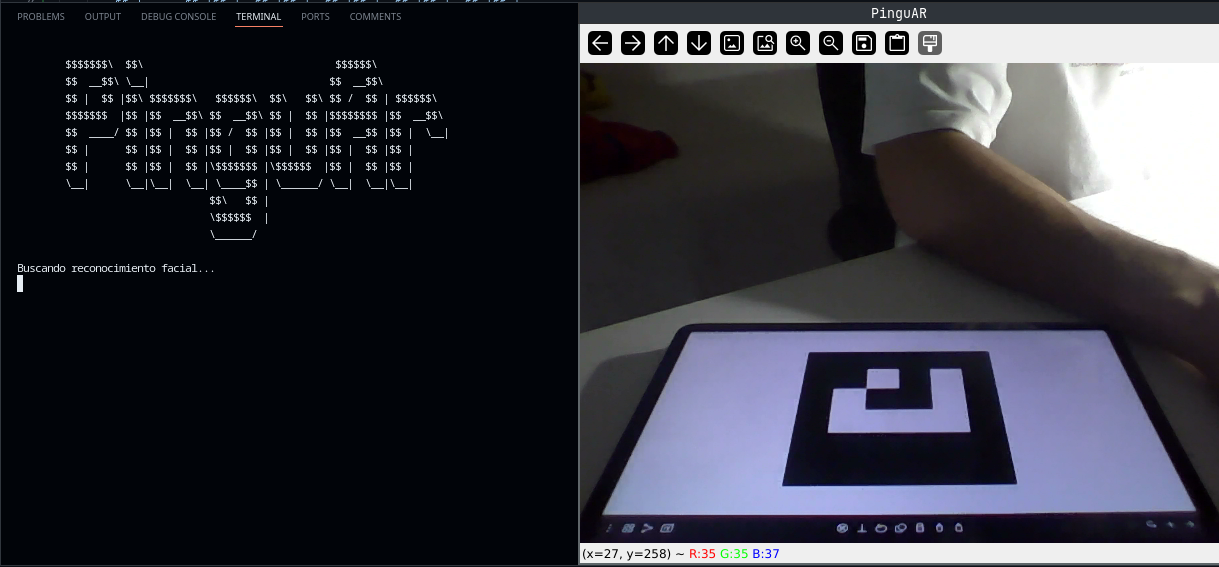
\includegraphics[width=0.8\textwidth]{./images/1.png}
	\caption{Reconocimiento Facial}
	\label{fig:Reconocimiento Facial}
	\end{figure}

	\newpage

    \item \textbf{Marcador Aruco:}
    
    Tras detectar la cara, se solicita al usuario que muestre el marcador Aruco número 1. Si el marcador es detectado, se muestra el modelo 3D del pingüino en la pantalla. La aplicación se estructura en tres escenarios:

	\item \textbf{Navegación entre Escenarios:}
    
    La navegación entre 3 escenarios se realiza mediante comandos de voz. Para ir al Escenario 1 se dice "UNO", para el Escenario 2 "DOS" y para el Escenario 3 "TRES". Cuando se está en el Escenario 2 o 3, se inicia el modo juego y se puede salir diciendo "SALIR", lo que permite volver a seleccionar otro escenario.

    \item \textbf{Detalles de los Escenarios:}
    
    - En el Escenario 1, el pingüino saluda al usuario por su nombre, muestra la hora, fecha, temperatura actual y su nivel de felicidad.
	\vskip 0.1in

	\begin{figure}[htbp]
		\centering
		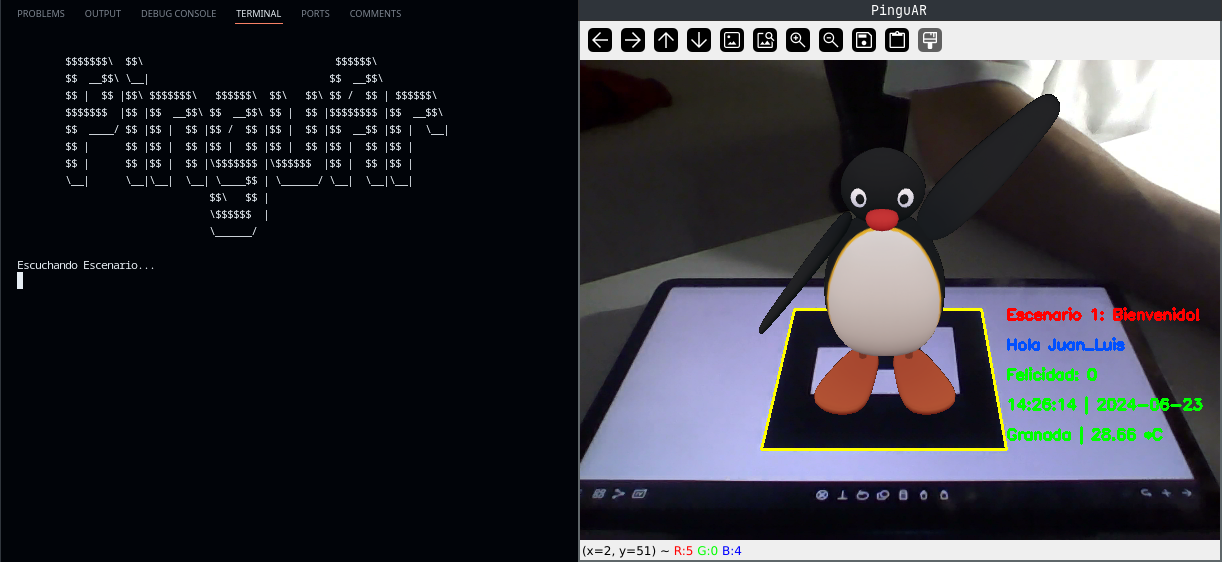
\includegraphics[width=0.9\textwidth]{./images/2.png}
		\caption{Escenario 1}
		\label{fig:Escenario 1}
		\end{figure}
    
	\newpage

	\vskip 0.1in
    - En el juego de alimentación (Escenario 2), decir "COME" hace que el pingüino coma, cuando este se llena aumenta su felicidad.
	\vskip 0.1in

	\begin{figure}[htbp]
		\centering
		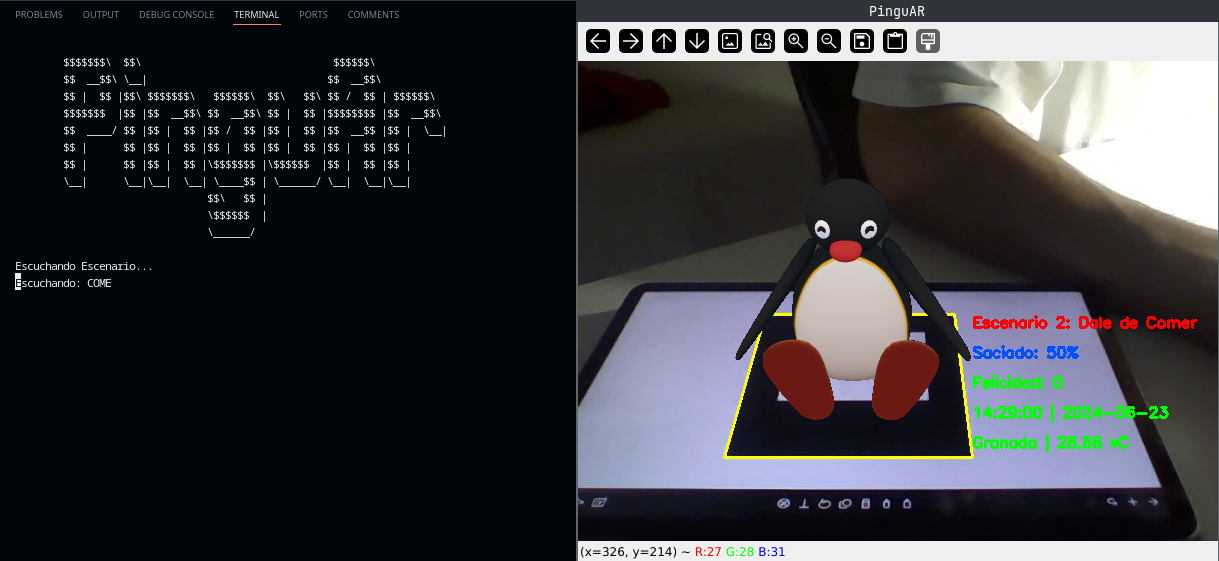
\includegraphics[width=0.9\textwidth]{./images/4.png}
		\caption{Escenario 2: Dandole de comer}
		\label{fig:Escenario 2}
		\end{figure}
		
	\begin{figure}[htbp]
		\centering
		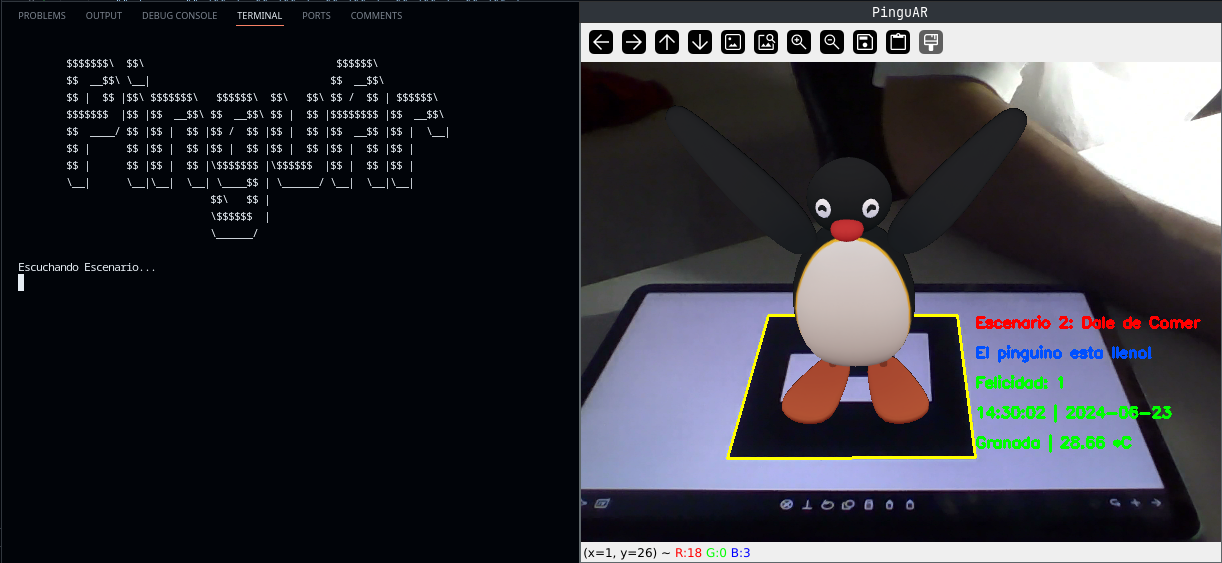
\includegraphics[width=0.9\textwidth]{./images/5.png}
		\caption{Escenario 2: Saciado}
		\label{fig:Escenario 2.1}
		\end{figure}	
    
	\newpage

	\vskip 0.1in
    - En el juego "¿Dónde está?" (Escenario 3), el pingüino se tapa la cara y el usuario debe preguntar "¿Dónde estás?". El pingüino reacciona al jugar con el, lo que aumenta su felicidad.
	\vskip 0.1in

	\begin{figure}[htbp]
		\centering
		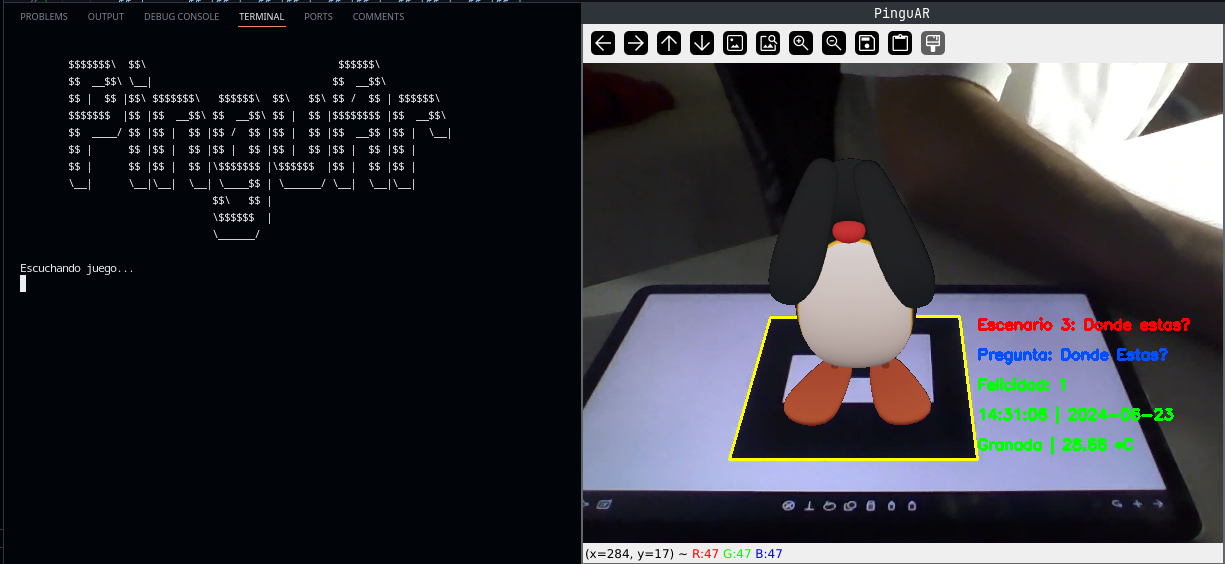
\includegraphics[width=0.9\textwidth]{./images/6.png}
		\caption{Escenario 3: ¿Donde está?}
		\label{fig:Escenario 3}
		\end{figure}

	\begin{figure}[htbp]
		\centering
		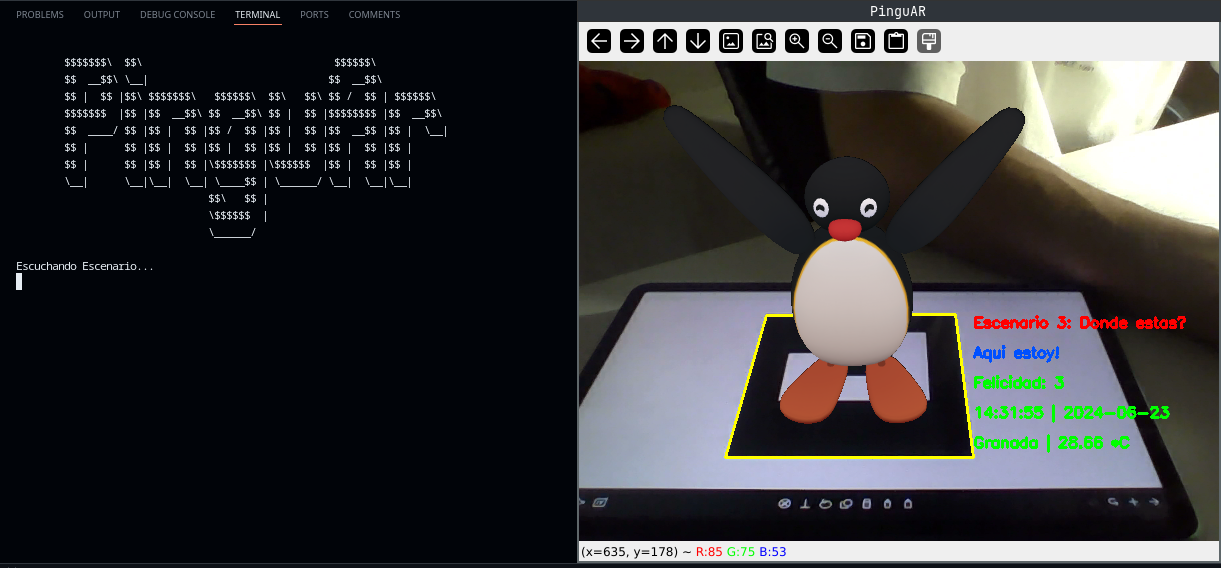
\includegraphics[width=0.9\textwidth]{./images/7.png}
		\caption{Escenario 3: Aqui esta}
		\label{fig:Escenario 3.1}
		\end{figure}
	
	\newpage



\end{enumerate}

\newpage

\section{Tecnologías Utilizadas en Computación Ubicua e Inteligencia Ambiental}

En el ámbito de la computación ubicua e inteligencia ambiental, se han utilizado diversas tecnologías para desarrollar esta aplicación, integrando características avanzadas como la realidad aumentada, el reconocimiento facial y el reconocimiento de voz.


\subsection{Realidad Aumentada}

    \begin{enumerate}
        \item \textbf{Marcadores ArUco:} 
        Se ha implementado el uso de marcadores ArUco debido a su robustez y fiabilidad en la detección y el seguimiento de objetos en entornos de realidad aumentada. 
		Los marcadores ArUco son una fácil identificación y posicionamiento de modelos 3D en el espacio real, proporcionando una experiencia inmersiva. En futuras versiones, 
		se pueden añadir más marcadores para representar simultáneamente múltiples modelos, decoraciones en la habitación y otros pingüinos, mejorando la interactividad y personalización del entorno, por lo 
		que su escalabilidad de cara al futuro es alta.

        \item \textbf{Representación del Modelo 3D:}
        Para la representación del modelo 3D del pingüino, se ha utilizado la librería \texttt{pyrender 0.1.45} en combinación con \texttt{trimesh 4.4.0}. 
		\texttt{Pyrender} facilita la renderización de modelos 3D de manera sencilla y eficiente, mientras que \texttt{trimesh} 
		proporciona herramientas para trabajar con mallas y geometrías complejas. Sin embargo, estas librerías presentan ciertas 
		limitaciones, como la falta de soporte para animaciones, lo cual restringe la capacidad de crear movimientos dinámicos y naturales en los modelos 3D, lo cual daria mas inmersion de la aplicacion.
		He creado los modelos con Blender, y los he exportado a formato glb, que es el formato que soporta pyrender. Se encuentran en la carpeta \texttt{media}
    \end{enumerate}

    \subsection{Reconocimiento Facial}

    Para el reconocimiento facial, se ha utilizado la librería \texttt{face-recognition 1.3.0}.
	 Esta librería, basada en \texttt{dlib}, es conocida por su precisión y facilidad de uso en la detección y 
	 comparación de rostros. He seguido una guía detallada para su implementación, disponible en
	 \newline
	  \texttt{https://www.youtube.com/watch?v=tl2eEBFEHqM}.

	\subsection{Reconocimiento de Voz}

    Para el reconocimiento de voz, se han utilizado las librerías \texttt{vosk 0.3.45} y \texttt{PyAudio 0.2.14}. 

    \begin{enumerate}
        \item \textbf{Vosk:} 
        Vosk es una herramienta de reconocimiento de voz que funciona offline, lo que garantiza la privacidad y 
		seguridad de los datos del usuario. Para su funcionamiento, se requiere la descarga de modelos específicos,
		 en este caso, el modelo \texttt{vosk-model-small-es-0.42}, disponible en este enlace \texttt{https://alphacephei.com/vosk/models}.

        \item \textbf{PyAudio:} 
        PyAudio se utiliza para la captura de audio desde el micrófono. Facilita la integración de entrada de audio en aplicaciones Python, asegurando una comunicación efectiva entre el usuario y la aplicación.
    \end{enumerate}

	\subsection{API de OpenWeather}
	Para obtener información meteorológica precisa y actualizada, 
	se ha utilizado la API de OpenWeather. 
	Esta API permite que el pingüino interactúe de manera dinámica con 
	nuestro entorno. Por ejemplo, se puede implementar una lógica condicional 
	donde, si la temperatura desciende por debajo de un cierto umbral, 
	el modelo del pingüino cambie su apariencia y muestre un mensaje relacionado con el frío.
	Igual con la hora, si es de noche, el pingüino se va a dormir, 
	si es de dia, se despierta,, con lo que conlleva cambiar sus respectivos modelos 
	y mensajes.

\vskip 0.1in
Estas tecnologías juntas hacen que la experiencia sea fluida y natural, siguiendo los principios de la computación ubicua. Permiten al usuario interactuar fácilmente con el entorno virtual del pingüino.

\newpage

\section{Cambios con respecto a la Entrega 1}

Inicialmente consideramos la idea de introducir cambios 
cosméticos para el pingüino. Sin embargo, desde mi perspectiva, 
implementar múltiples modelos 3D requeriría mucho tiempo y 
complicaría la diferenciación visual entre el pingüino y sus
cosméticos en la escena. Por esta razón, hemos decidido 
mantener al pingüino como el personaje principal y en lugar de eso,
agregarle más funcionalidades.
\vskip 0.1in
No he podido implementar botones debido a limitaciones en 
\texttt{pyrender}. He visto que hay frameworks mas intuitivos y preparados 
para enotrnos de realidad virtual con Unity y Vuforia
 Es más práctico realizar interacciones a 
través del reconocimiento de voz. Para representar el cuidado 
del pingüino a lo largo del tiempo, he optado por utilizar una 
variable de felicidad como métrica principal donde nuestro objetivo es 
maximizar la felicidad del pingüino jugando con el.
\vskip 0.1in
La idea de que el pingüino crezca podría implementarse 
cambiando su modelo por uno más grande según ciertos criterios
 como la hora del día. Sin embargo, la implementación de 
 variaciones basadas en la hora y temperatura actual no 
 está disponible actualmente debido a la necesidad de crear 
 y añadir más modelos 3D, lo cual requiere más tiempo del que
  he podido dedicar hasta ahora. En este proyecto me he centrado más en las funcionalidades relacionadas con la representacion del modelo,
  reconocimiento de voz y facial antes que la creacion de modelos 3D en Blender.


\end{document}